\section{Model i konstrukcja skanera 3D}
W celu wykonania dokładnych modeli trójwymiarowych został utworzony skaner 3D na podstawie autorskiego projektu. W skład zestawu wchodzi kamera Intel RealSense D435i oraz platforma obrotowa. Wybór sensora od firmy Intel nie był przypadkowy. Posiada on szereg wbudowanych funkcji, takich jak łatwa możliwość kalibracji oraz nastaw odpowiednich parametrów wykrywania głębi. Jego rozdzielczość oraz dostępna liczba klatek na sekundę sprawia, że akwizycja danych jest o wiele dokładniejsza. Podczas budowy skanera dokonano porównania możliwości dwóch kamer trójwymiarowych: Intel RealSense D435i oraz Orbbec Astra Mini MX6000. W tabeli ~\ref{tab:intelvsorbbec} dokonano przeglądu najważniejszych charakterystyk obu tych skanerów, zestawiono między innymi rozdzielczości głębi oraz kąt przechwytywania obrazu.

\begin{table}[H]
\begin{center}

\caption{\label{tab:intelvsorbbec}Porównanie charakterystyk kamer Intel RealSense D435i oraz Orbbec Astra Mini MX6000 \cite{OrbbecAstraMiniSheet} \cite{IntelRealSenseSheet}.}
\centerline{
\begin{tabular}{ |c| c|c| }
 \hline
 {\small Kamera} & {\small Astra Mini} & {\small RealSense D435i}\\ 
 \hline
 {\small Dokładność} & {\small $\pm$ 1-3mm na 1 m} & {\small < \text{2\%}  na 2 m}\\ 
  \hline
   {\small FOV} & {\small 60 \degree H x 49.5 \degree V} & {\small 87 \degree H x 58 \degree V}\\ 
  \hline
 {\small Rozdzielczość RGB } & {\small 640 px x 480 px } & {\small 1920 px x 1080 px}   \\  
  \hline
   {\small Rozdzielczość głębi } & {\small 640 px x 480 px } & {\small 1280 px x 720 px }   \\  
  \hline
     {\small FPS } & {\small 30} & {\small 90}   \\  
  \hline
   {\small  Długość fali lasera } & {\small 830 nm} & {\small 850 nm}  \\  
  \hline
\end{tabular}
}
\end{center}
\end{table}
Z powyższych charakterystyk wynika, że kamera firmy Intel jest dokładniejsza oraz lepiej spełni zadanie wiernego odwzorowania modelu 3D. Ponadto oprogramowanie dostarczane przez firmę Intel o nazwie RealSense Viewer pozwala na łatwą obsługę tego urządzenia. Umożliwia ono podgląd obrazu z kamery zarówno w 2D jak i w 3D. W programie dostępne są ustawienia, umożliwiające poprawną regulację parametrów rejestracji obrazu, takie jak moc lasera, wartość graniczną wykrywanej głębi oraz ekspozycję. Wszystkie te aspekty znacząco usprawniają proces kalibracji, produktywność oraz wpływają na poprawę dokładności generowanych obrazów.
Konstrukcja zbudowanego skanera została zaprezentowana na rysunku ~\ref{fig:konstrukcjaModelu}. 
\begin{figure}[H]
  \centering
    \includesvg[scale=0.75]{modelSkanera.svg}
  \caption{Schemat budowy autorskiego skanera 3D.}   
  \label{fig:konstrukcjaModelu}
\end{figure}
Na powyższym rysunku można dostrzec dwa kluczowe elementy wchodzące w skład skanera. Platforma ruchoma napędzana silnikiem elektrycznym zapewnia stałą prędkość kątową obrotu tacki. Dzięki temu wyznaczanie położenia obiektu w przestrzeni jest dokładne. Wykonane zostały testy platformy napędzanej silnikiem elektrycznym oraz poruszanej ręcznie. Z wytworzonych w ten sposób modeli wynika jasno, iż stała prędkość kątowa obiektu jest kluczowa do poprawnego przekształcenia modelu. Kolejnym elementem wykorzystanym przy budowie skanera jest kamera RGBD. Wykonuje ona zdjęcia kolorowe oraz głębi z określoną częstotliwością oraz zapisuje je do pliku, w celu późniejszej ich obróbki. Ze względu na wykorzystanie platformy o stałej prędkości kątowej, dokonane zostało porównanie wpływu FPS na wygląd ostatecznego modelu. Zmiana liczby klatek na sekundę wpływa bezpośrednio na rozdzielczość kątową wykonanych zdjęć, gdy ta liczba jest większa, gęstość chmury punktów również się zwiększa.\\
\indent Zasada funkcjonowania skanera została przedstawiona poniżej:
\begin{enumerate}
    \item Mierzona jest dokładna odległość obiektywu kamery od środka tacki.
    \item Obiekt umieszczany jest na obrotowej tacce.
    \item Dokonuje się kalibracji tak ustawionego elementu, tak by stopień wypełnienia punktów był jak najdokładniejszy.
    \item Tacka zostaje uruchomiona z prędkością 0.1 $\frac{rad}{s}$.
    \item Uruchomiony zostaje zapis obrazu głębi oraz RGB z kamery.
    \item Gdy tacka wykona pełen obrót, nagrywanie oraz tacka zostają zatrzymane. 
\end{enumerate}

Wysokość obiektu jest mierzona na podstawie danych z kamery RGBD. Znając odległość kamery od obiektu, można wyznaczyć jego wysokość korzystając ze wzoru:

\begin{equation}
    \begin{aligned}
        H_{m}=D\cdot \frac{h_{pix}}{h_{sens}}\cdot V_{FOV}
    \end{aligned}
\label{equ:wysokoscRealPix}
\end{equation}
W powyższym wzorze $H_{m}$ jest rzeczywistą wysokością obiektu, D określa odległość kamery od obiektu w metrach, zaś $V_{FOV}$ oznacza pionowy kąt widzenia kamery. Wysokość soczewki kamery została oznaczona we wzorze jako $h_{sens}$, a $h_{pix}$ jest wysokością obiektu w pikselach. 

W celu wyznaczenia rzeczywistej wysokości obiektu w zależności od odległości i jego wysokości w pikselach, należy znać pionowy kąt widzenia kamery oraz wysokość soczewki. Informacje o kącie widzenia skanera znajdują się w dokumentacji urządzenia Intel RealSense D435i, natomiast wysokość soczewki należy wyznaczyć empirycznie \cite{IntelRealSenseSheet}. W tym celu, dokonano pomiaru wysokości obiektu w pikselach na obrazie z kamery oraz jego odległość od obiektywu. Badanie powtórzono 8 razy w celu uzyskania dokładnej aproksymacji. Znając odległość oraz rzeczywistą wysokość obiektu, po przekształceniu wzoru można uzyskać wartość $h_{sens}$. Po uśrednieniu wyników ze wszystkich pomiarów przeprowadzono badanie jakości estymacji wysokości. Wykres rzeczywistej wysokości obiektu oraz jej przybliżenia znajduje się na rysunku ~\ref{fig:wysokoscOdleglosc}.
\begin{figure}[H]
  \centering
    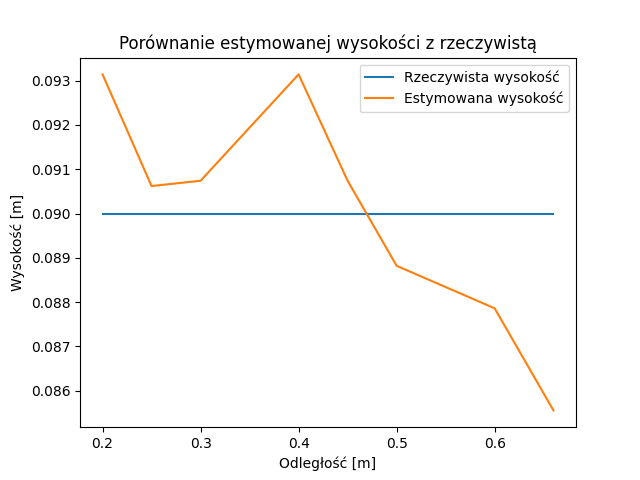
\includegraphics[scale=0.55]{wysokoscPredykcja.png}
  \caption{Porównanie rzeczywistej wysokości z jej estymacją.}   
  \label{fig:wysokoscOdleglosc}
\end{figure}
Na powyższym rysunku można zauważyć, że aproksymacja wysokości daje dobre rezultaty. W zakresie od 20 cm do 66 cm, maksymalny błąd względny wyniósł 4.2\%. Otrzymane rezultaty są zadowalające do poprawnej wizualizacji rzeczywistego obiektu.
